The Monte Carlo technique has been a widespread method for simulating liquid crystals and molecular dynamics at large. With credit generally awarded to John von Neumann, Stanislaw Ulam, and Nicholas Metropolis, the method was devised in the late 1940's as part of the Second World War effort by studying the diffusion of neutrons in fissionable material (\cite{allenbook} pg.\ 147). The principle is to treat a determinate mathematical problem with a probabilistic analogue and solve it by stochastic sampling. More specifically, we use the Metropolis Monte Carlo method published in 1953 by Metropolis \textit{et al.}\ \cite{metropolis1953}.

The method aims to explore the state space, while also tending towards states of higher statistical probability. We let $t$ count the number of ``Monte Carlo Steps'' (MCSs), where one MCS attempts $N$ random movements of molecules, either by iterating over the molecule list or randomly selecting $N$ molecules, though Ref.\ \cite{hastings1970} found iterating over the list equally valid with the benefit of being that bit simpler. We also let $\bv{\Gamma}(t)$ represent the system state at time step $t$, with $\bv{\Gamma}(0)$ being the initial state. In the case of our liquid crystal system of hard rods, a random rod movement would mean
\begin{align}
	\bv{r}_i(t+1) &= \bv{r}_i(t) + \delta\bv{r}\\
	\theta_i(t+1) &= \theta_i(t) + \delta\theta
	\label{eq:mcmoves}
\end{align}
for rod label $i$, and small spatial and angular displacements $\delta\bv{r}$ and $\delta\theta$. 
In the Metropolis algorithm, we must create a rule for the acceptance or rejection of a proposed move. We start by considering abstractly the state energy at time $t$, $E(t)$. The first condition in our rule is that if $E(t+1) < E(t)$, then this is energetically favourable and we accept the move (postponing the calculation of $E(t)$ for now). In the case of $E(t+1) > E(t)$ we do not flat out reject this. Instead we consider the Boltzmann factor, that is the probability of the system being in state $\bv{\Gamma}(t+1)$:
\begin{align}
	p_\Gamma(t+1) &= \frac{1}{Z}e^{-E(t+1)/k_BT}
\end{align}
with the canonical partition function $Z$. 
Further, we may compare the probability of this state with $\bv{\Gamma}(t)$ 
\begin{align}
	\nonumber
	\frac{p_\Gamma(t+1)}{p_\Gamma(t)} &= 
	\frac{e^{-E(t+1)/k_BT}}{e^{-E(t)/k_BT}}\\
	&=e^{-(E(t+1) - E(t))/k_BT} = e^{-\Delta E/k_BT}.
	\label{eq:pGamma}
\end{align}

We then base the decision of acceptance/rejection off this relative probability. To do so, a random number $\varepsilon$ is generated in the range $0\leq \varepsilon \leq 1$, and compared with the probability ratio $p_\Gamma(t+1)/p_\Gamma(t)$. The rule is to accept the proposed move if $\varepsilon < p_\Gamma(t+1)/p_\Gamma(t)$. 

\begin{figure}
	\centering
	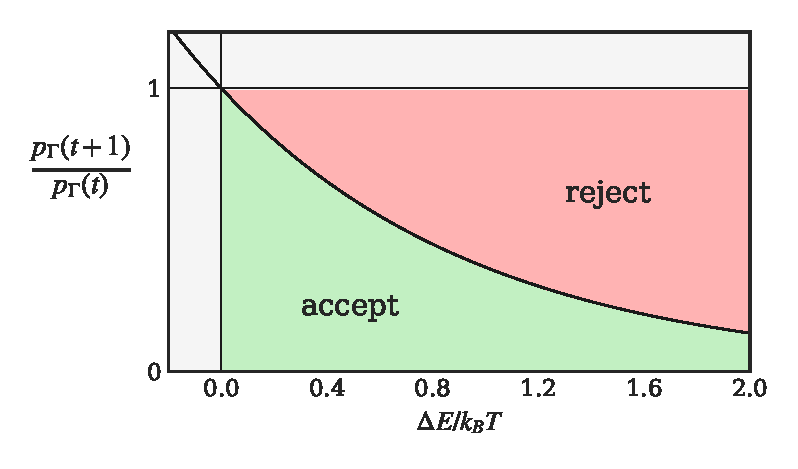
\includegraphics[width=0.8\textwidth]{mc_accrej.eps}
	\caption{Probability ratio of Eq.\ \ref{eq:pGamma} showing chances of acceptance or rejection upon generating $\varepsilon$ for a given $\Delta E$.}
	\label{fig:accrej}
\end{figure}

Figure \ref{fig:accrej} shows the chances of acceptance/rejection of a move for a given $\Delta E$. Moves that are energetically costly always have a finite chance of being accepted, though it is exponentially unlikely as $\Delta E$ increases. This feature is essential for the simulation to explore the phase space properly. Notice also that the acceptance approaches unity as $\Delta E \rightarrow 0$ as we expect.\\

In calculating $\Delta E/k_BT$, we needn't calculate the total system energies $E(t)$ and $E(t~+~1)$, rather since we only need their difference we simply calculate the energy change associated with the proposed move. As described in Ref.\ \cite{allenbook} pg.\ 156, the change in potential energy is calculated by summing over the interaction energies, $\epsilon_{ij}$, between our selected molecule $i$ and the other relevant molecules $j$,
\begin{align}
	\Delta E = \sum_j \epsilon_{ij}(t+1) - \sum_j \epsilon_{ij}(t).
\end{align}
This also has the advantage that interactions beyond a certain cutoff distance for both molecular positions, such as a mean field, cancel each other out.

Returning to our liquid crystal model of steric rods, the situation gains a simplification. Recall that the interaction potential of neighbouring molecules is approximated as a delta function: it is zero everywhere except for if there is an overlap at which point it is infinite. Thus, when a proposed move causes an overlap this results in $\Delta E = +\infty$, and conversely if the move grants no overlap, the system perceives no change in potential energy and $\Delta E = 0$. As these are the only two scenarios, we may circumnavigate the entire $\varepsilon$ generation and comparison phase, with an overlap having no probability of success and a non-overlap always being accepted.

It is up to the simulator to determine which magnitudes of $\delta\bv{r}$ and $\delta\theta$ from Eq.\ \ref{eq:mcmoves}  work best for their system. There is no theoretic solution for an optimal choice (\cite{allenbook} pg.\ 159). Generally, the smaller a degree of movement, the more likely a move is to be accepted. However, there is an inverse consequence in that the system generally explores the phase space more slowly. 
As briefly discussed in Allen \& Tildesly (\cite{allenbook} pg.\ 159), often simulators will choose a failure rate of around $0.5$, but a study by Ref.\  \cite{wood1959} found $0.9$ maximized the root-mean-square displacement of atoms as a function of computer time. Allen \& Tildesly soundly point out though, this study was carried out on a first generation computer (1959), with 32 hard spheres at a particular packing fraction, and there is no reason to believe that their optimum is universal, or even that root-mean-square displacement is always the desired metric for phase space exploration.

